\begin{figure}[ht]
\centering
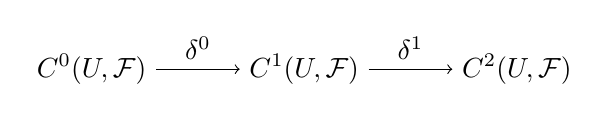
\begin{tikzpicture}[node distance=2.7cm]
  \node (C0) {$C^0(\mathfrak U,\mathcal F)$};
  \node[right of=C0] (C1) {$C^1(\mathfrak U,\mathcal F)$};
  \node[right of=C1] (C2) {$C^2(\mathfrak U,\mathcal F)$};
  \draw[->] (C0) -- node[above] {$\delta^0$} (C1);
  \draw[->] (C1) -- node[above] {$\delta^1$} (C2);
\end{tikzpicture}
\caption{The \v{C}ech cochain complex associated with an open cover.}
\end{figure}
